\subsection{Providing Access Control}
This section aims to show how the yellow system handles requests from clients based on which actor they represent. AutoSys is a multi-user system with a manager and researcher actor. A researcher can both be assigned the role of a reviewer and validator since only their tasks are different. We have drawn an access control matrix depicting the allowed operations on the entity objects for both actors. In summary, a Manager can create Users and Teams while Researchers can create Studies and receive Tasks. Ideally, all actors must first be authenticated based on their role before they can modify any object in the system. One would then use access control lists on each object to check the access privileges of the user. 
Below is the access matrix for main AutoSys objects. Note that the study object is comprised of a StudyReport, ResearchProtocol and a Phase with Criteria. Tasks are generated in a Phase. Also, we have omitted method names for Users and Teams that only have CRUD operations. Finally, we assume that a Manager cannot also be a Researcher. 

\begin{figure}[H]
	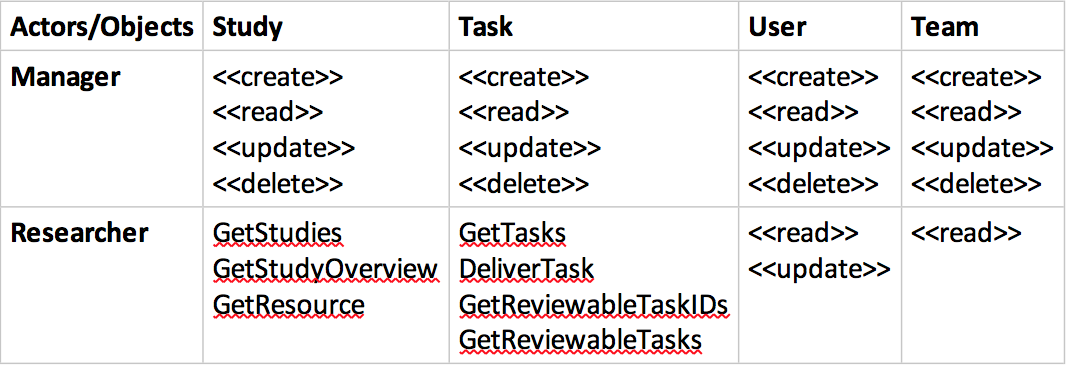
\includegraphics[width = \linewidth]{Images/accessmatrix}
	\caption{Access matrix for main AutoSys objects}
	\label{fig:accessmatrix}
\end{figure}